\section{System Operation Chart}
\label{sec:operatingChart}

Operating charts describe the modes of operation and the flow of the system without much detail. Figure~\ref{fig:systemFlowchart} shows a state diagram of the system's operation that depicts all available operating. It shows the course of action taken by the software when a complete experiment is performed. A general but brief overview of the different modes of operation follows.

\begin{figure}[!ht]
	\centering
	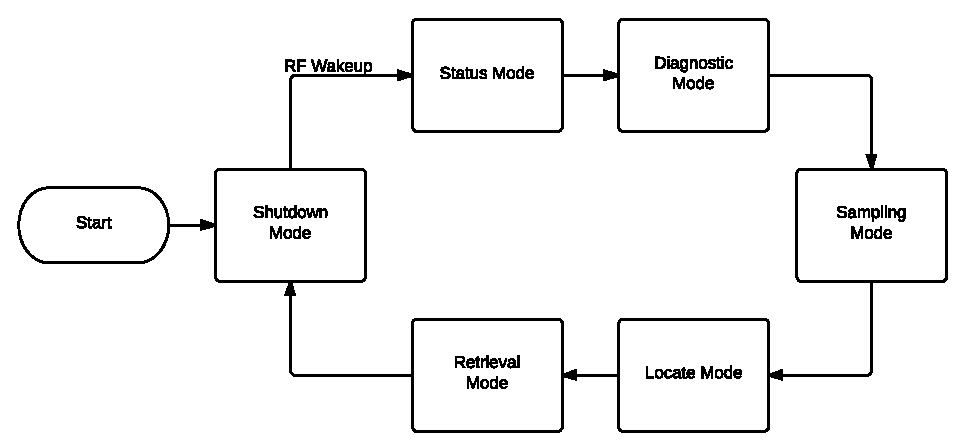
\includegraphics[width=\textwidth]{img/stateDiagram}
	\caption{Software state diagram depicting all available operating modes. \label{fig:systemFlowchart}}
\end{figure}

When the system is powered up it performs an initialization sequence, which includes initializing all GPIO ports and memory variables. It also enables global interrupts and the RF wakeup receiver interrupt while keeping all other interrupts disabled. Subsequently all other modules except the RF wakeup receiver are powered down.

Once the initialization sequence is finished, the system enters a very low power mode, called shutdown mode.  The system can be woken up by the RF wakeup receiver which is listening for a specific signal from the user. When the system is interrupted from sleep by the RF wakeup receiver it powers on the XBee module, establishes a ZigBee connection, and enables the XBee interrupt. Additionally, the system powers down the RF wakeup receiver and disables its corresponding interrupt.

Afterwards, the system enters another low power mode which is referred to as standby mode. In this mode, the system maintains an active ZigBee connection via the XBee module. At this point, the XBee module is listening for specific signal from the base station. When it receives a signal, it interrupts the MCU and sets a flag corresponding to the signal that was received. The signals received meant are meant to switch between diagnostic, retrieval, sampling, status, locate or shutdown mode. A signal can also tell the drifters to exit diagnostic mode or to exit locate mode. The interrupt routine then takes the CPU to active mode, and the system proceeds to execute the service corresponding to the signal that was sent to the XBee module via the base station. After the service has finished executing, the system returns to standby mode where it listens for more incoming commands.